\author{PREN Gruppe 7}
\title{Silisloth}
\subtitle{Dokumentation PREN 2}
\date{\today}

\begin{multicols}{2}
\maketitle
\columnbreak
    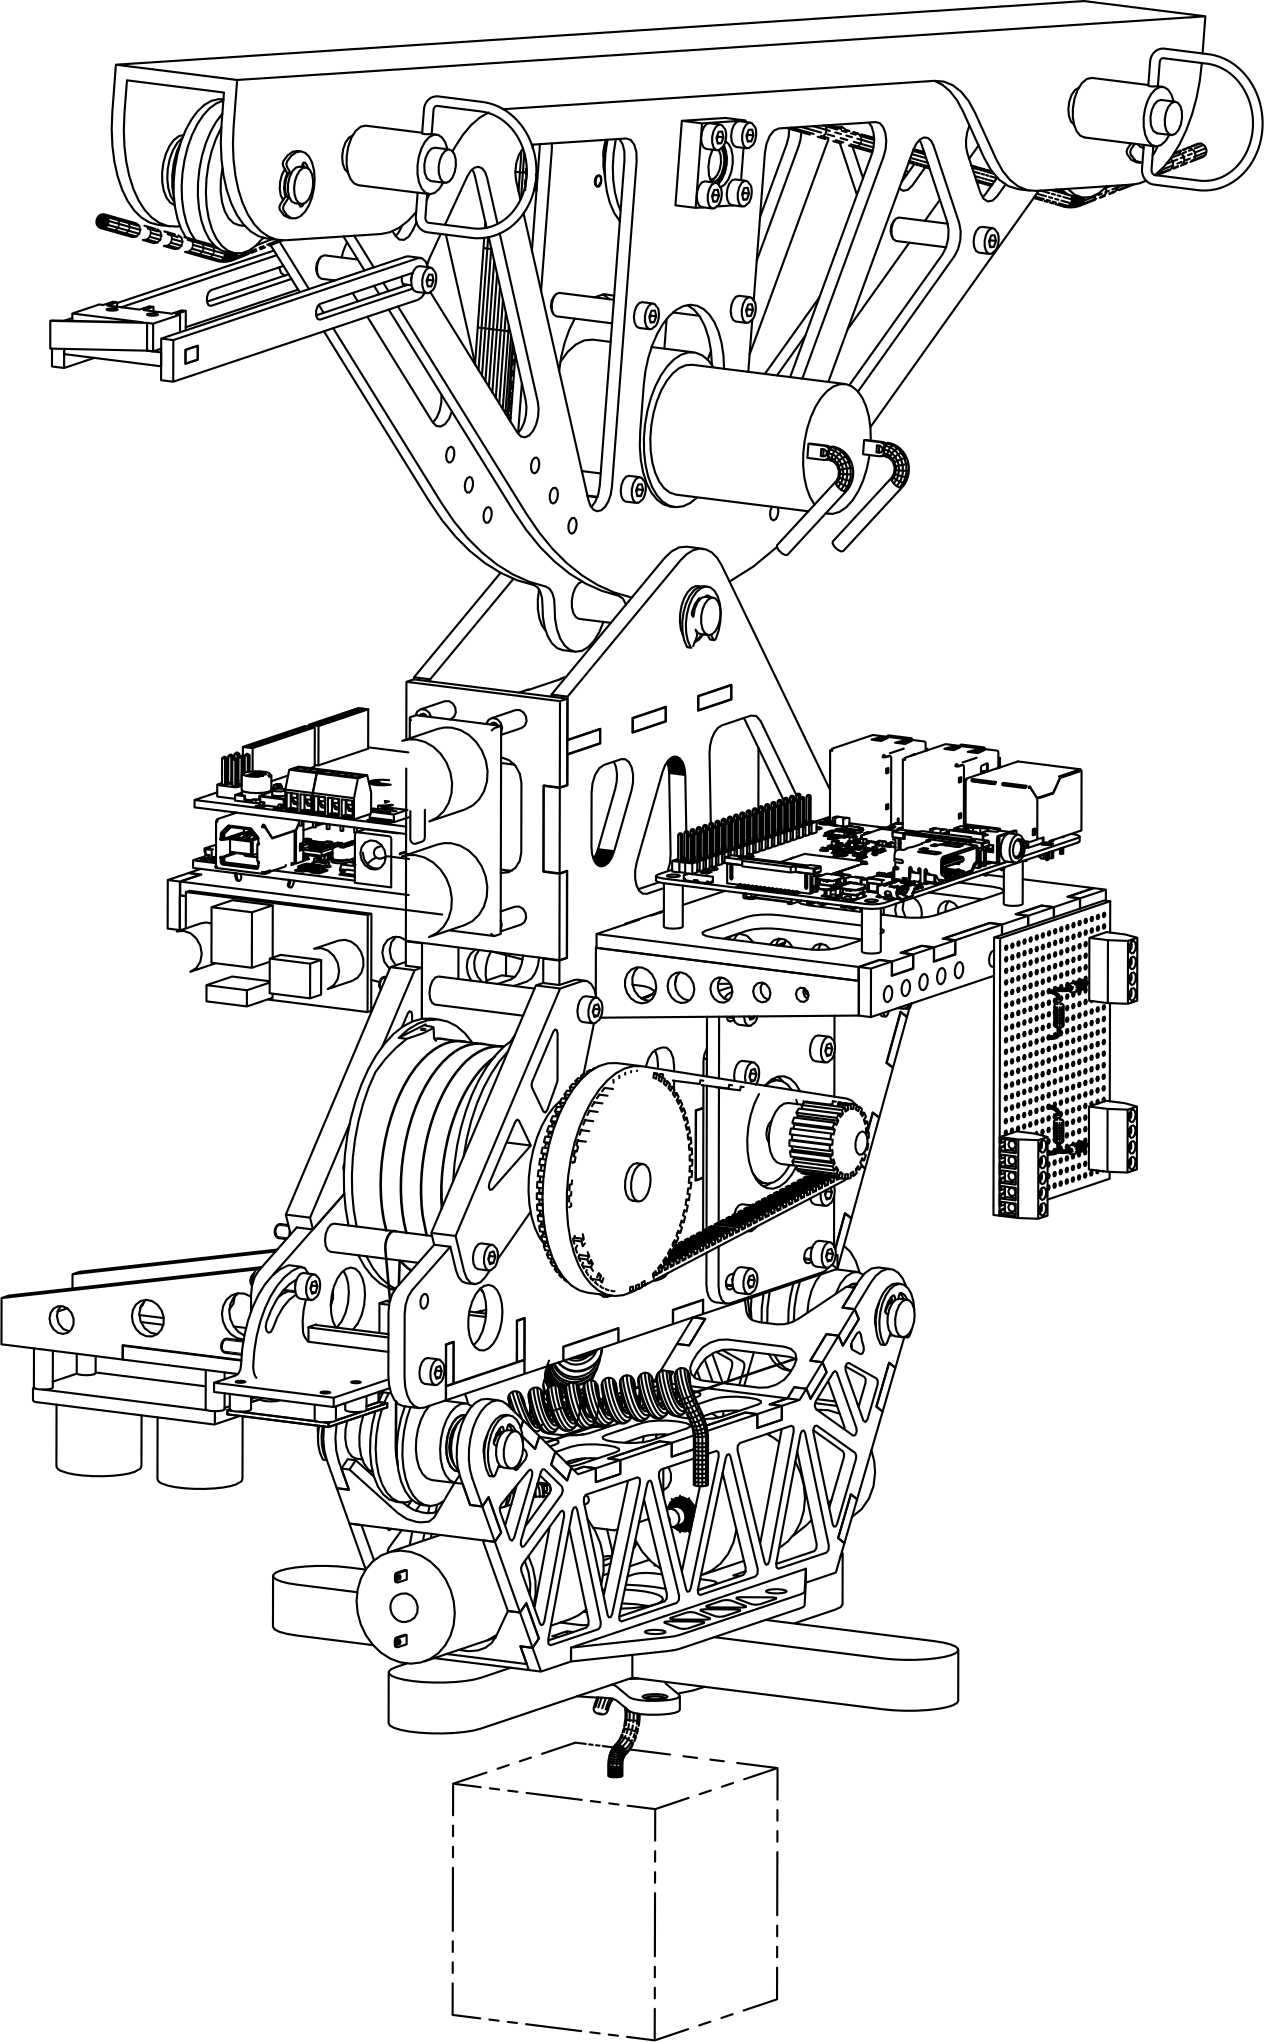
\includegraphics[width=0.75\columnwidth]{pics/assembly-schraeg.png}
\end{multicols}

\section*{Versionierung}
\def\arraystretch{1.2}
\begin{tabularx}{\textwidth}{|r|l|X|}
\hline
\textbf{Version} & \textbf{Datum} & \textbf{Bemerkung} \\
\hline
0.1 & Fr, 23.03.2018 & Aufsetzen des Dokuments \\
0.2 & Fr, 25.05.2018 & Fertigstellung der Vorabversion \\
1.0 & Fr, 10.06.2018 & Fertigstellung für Schlussabgabe \\
\hline
\end{tabularx}
\vspace{1em}

\begin{multicols}{2}
\section*{Betreuer}
Zeno \textsc{Stössel}, Elektrotechnik
\section*{Experten}
Jörg \textsc{Hofstetter}, Informatik \\
Carsten \textsc{Haak}, Maschinentechnik
\vfill\null
\columnbreak
\section*{Autoren}
Sandro \textsc{Bertozzi}, Informatik \\
Christoph \textsc{Binkert}, Maschinentechnik \\
Patrick \textsc{Bucher}, Informatik \\
Alex \textsc{Duong}, Elektrotechnik \\
Quentin \textsc{Frei}, Maschinentechnik \\
Jan \textsc{Greber}, Elektrotechnik \\
Marko \textsc{Lovrinovic}, Maschinentechnik \\
Johannes \textsc{Togan}, Maschinentechnik
\end{multicols}
